\documentclass[11pt]{article}
\usepackage[margin=1in]{geometry}
\usepackage{graphicx}
\usepackage{microtype}
\usepackage{verbatim}
\usepackage{amsmath}
\usepackage{nicefrac}
\usepackage[colorlinks=false, pdfborder={0 0 0}]{hyperref}
\begin{document}
\title{Rudder Controller \& Wiper Controller\\Embedded System Design, Lab 2}
\date{September 25, 2015}
\author{Ben Lorenzetti}
\maketitle
\tableofcontents

\clearpage

\section{Objectives and Problem Description}

The primary objective of this lab was learning to interface with two new types of peripherals: a servo motor and potentiometers.
Several new functions in PBASIC are introduced for these types of actuators and transducers.

\subsection{Rudder Controller}

Control the angular position of a tiny ship's rudder (i.e. the horn of your servo)
based on the input from a steering wheel (i.e. your potentiometer).
The full range of motion of the ship's rudder should be $45^{o}<\theta<135^{o}$
and it should be controlled linearly by the full range of the potentiometer.

\subsection{Wiper Controller}

Instead of controlling angular position, as was done for the rudder controller,
use the potentiometer to control the angular velocity of the servo.
The servo represents a single windshield wiper, and should rotate continuously
between $15^{o}$ and $160^{o}$. The full range of the potentiometer should
be used to linearly control the wiper speed from 0 degrees/sec up to the
maximum speed.

\section{Procedure}
\subsection{Assignment: Ch. 4 Servo Motor}

To prepare for this lab, we were instructed to read chapters 4 and 5 in the Parallax What's a Microcontroller book and complete the example activities.

The parallax servo motor has three connectiong: power, ground, and signal.
The signal (white) connection is used to control the angular position of
the horn, from $0^{o}$ to $180^{o}$.
The servo expects a square wave control signal,
where the period is approximately 20 ms
and the width of the high pulse carries angular displacement information.

\begin{figure}[h!]
\centering
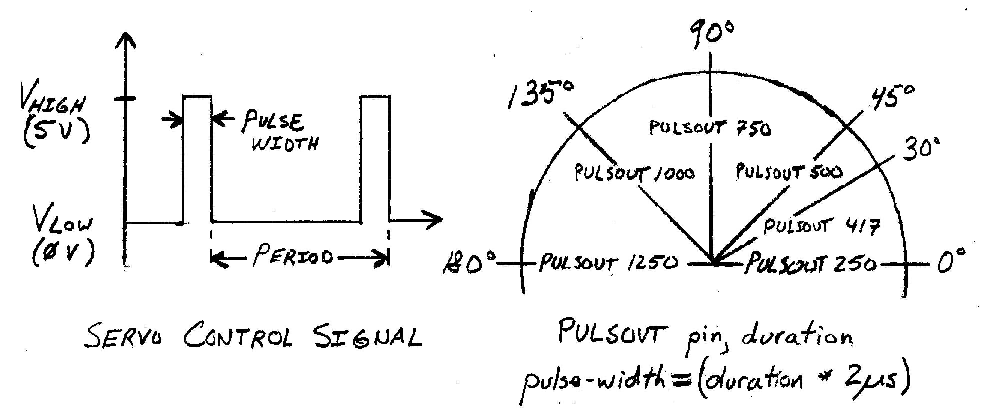
\includegraphics[width=0.8\textwidth]{pulse-width-vs-angular-displacement.pdf}
\caption{Servo Control Signal Timing}
\label{pulse-width-vs-angular-displacement}
\end{figure}

The formula relating pulse width and angular displacement is
\begin{equation}
t_{p-width}(\theta)=\left\{\begin{array}{c c}
\frac{250\mu s}{45^{o}}\theta+250\mu s	&	10^{o}<\theta<170^{o}\\
0\mu s	&	\textrm{servo off}	\\
\end{array}\right.
\label{pulse-width-eq}
\end{equation}

The function for doing pulse width modulation in PBASIC is
\texttt{PULSOUT pin, duration}, where \texttt{pin} is the
I/O port number and \texttt{duration} is the length of time high.
Of course, since this Stamp and PBASIC, the board isn't quite
fast enough so \texttt{duration} is in units of $2\mu s$ and
you have to complete the pulse width modulation yourself by
\texttt{PAUSE}ing for 20 ms, or however long the period should
be approximately.

To avoid dealing with PBASICs strange limitations,
we can rewrite equation \ref{pulse-width-eq} as
\begin{equation}
\textrm{duration}=\frac{25}{9}*\theta+125, \quad 10^{o}<\theta<170^{o}
\end{equation}

Chapter 4 also provided two more expressions in PBASIC that are helpful with servo motors:
\begin{verbatim}
i VAR Word
FOR i = 0 TO 150
	...
LOOP
}
\end{verbatim}
and
\texttt{duration = duration MIN 350 MAX 1150}.

\subsection{Assignment: Ch.5 Potentiometers}

Not surprisingly, the Basic Stamp is too primative to have an analog-to-digital converter,
so you can only measure analog inputs with a function called \texttt{RCTIME},
and then only if you construct an RC decay circuit--and again only if the input
signal is stable for a long enough charging time and can source enough current.

The function prototype is \texttt{RCTIME pin, state, duration},
where \texttt{pin} is the I/O pin number (0-15), \texttt{state} is the
expected charged status of the pin (0 or 1), and \texttt{duration} is
a variable to store the decay time--in units of $2\mu s$.
The decay time is taken when the voltage on \texttt{pin} falls below
$1.4V$, if the original charge \texttt{state} was 1.

\begin{figure}[h!]
\centering
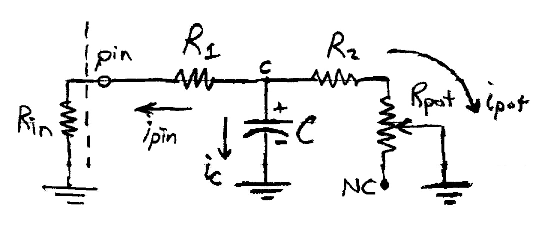
\includegraphics[width=0.5\textwidth]{pot-input-circuit.pdf}
\caption{Input Circuit for Reading a Potentiometer with \texttt{RCTIME}}
\label{pot-input-circuit}
\end{figure}

An input source that is well suited to \texttt{RCTIME} is a rotary
potentiometer. A circuit combining a potentiometer and capacitor is shown
if \hyperref[pot-input-circuit]{figure \ref{pot-input-circuit}}.

If we assume infinite input resistance once \texttt{RCTIME} switches
the pin direction to input, then $i_{pin}=0$ and $V_{in}=V_{c}$.
Taking Kirchoff's Current Law at node c allows us to solve for input
voltage as a function of time and initial condition across C.
\begin{equation*}
i_{pin}+i_{c}+i_{pot}=0
\end{equation*}
\begin{equation*}
0+C\frac{dV_{in}}{dt}+\frac{V_{in}}{R_{2}+R_{pot}}=0
\end{equation*}
\begin{equation*}
\frac{-V_{in}}{R_{2}+R_{pot}}=C\frac{dV_{in}}{dt}
\end{equation*}
\begin{equation*}
\frac{-1}{C(R_{2}+R_{pot})}*dt=\frac{1}{V_{in}}*dV_{in}
\end{equation*}
\begin{equation*}
\frac{-t}{C(R_{2}+R_{pot})}+A=ln(V_{in})
\end{equation*}
\begin{equation*}
e^{ln(V_{in})}=e^{\frac{-t}{C(R_{2}+R_{pot})}}
\end{equation*}
\begin{equation*}
V_{in}=e^{A}*e^{\nicefrac{-t}{C(R_{2}+R_{pot})}}
\end{equation*}
\begin{equation}
V_{in}(t)=V_{0}e^{-t/\tau} \quad \quad \tau=(R_{2}+R_{pot})C
\label{rc-decay-eq}
\end{equation}

Using equation \ref{rc-decay-eq}, the decay time required to discharge
from $V_{HIGH}$ to $V_{LOW}$ is
\begin{equation*}
V_{LOW}=V_{HIGH}e^{\nicefrac{-t_{discharge}}{\tau}}
\end{equation*}
\begin{equation*}
t_{discharge}=\tau*ln\left(\frac{V_{HIGH}}{V_{LOW}}\right)
\end{equation*}
For $V_{HIGH}=5V$, $V_{LOW}=1.4V$, $C=3,300\mu F$, this evaluates to
\begin{equation}
t_{discharge}=\left[\frac{2.1}{10^{3}}*\frac{2\mu s}{\Omega}\right]*(R_{2}+R_{pot})
\label{t-discharge-eq}
\end{equation}

A $10k\Omega$ potentiometer with $R_{2}=220\Omega$, leads to input
domain $220\Omega<R_{2}+R_{pot}<10.22k\Omega$ and output range
$0.462*2\mu s<t_{discharge}<21.462*2\mu s$. When we consider
that the PBASIC Stamp board only has an integer resolution of
$2 \mu s$, then the expected result from a call to
\mbox{\texttt{RCTIME, pin, 1, duration}} is in the set
\begin{equation}
\textrm{\texttt{duration}}=\{1, 2, 3,..., 21, 22\}
\end{equation}
when the 10 k$\Omega$ potentiometer is used with a 3,300 $\mu F$ capacitor.

\subsection{Traffic Light Controller}

The lab said to go through the first 3 chapters of the book and do the activities, so I did this.

I built the circuit shown in \hyperref[traffic-light-circuit]{figure \ref{traffic-light-circuit}} on the Basic Stamp breadboard.
It has the 6 LEDs in active low configuration with $1k\Omega$ current limiting resistors.
The pushbutton switch was also configured active low for consistency.
It also has a $1k\Omega$ current limiting resistor.

\begin{figure}[h!]
\centering
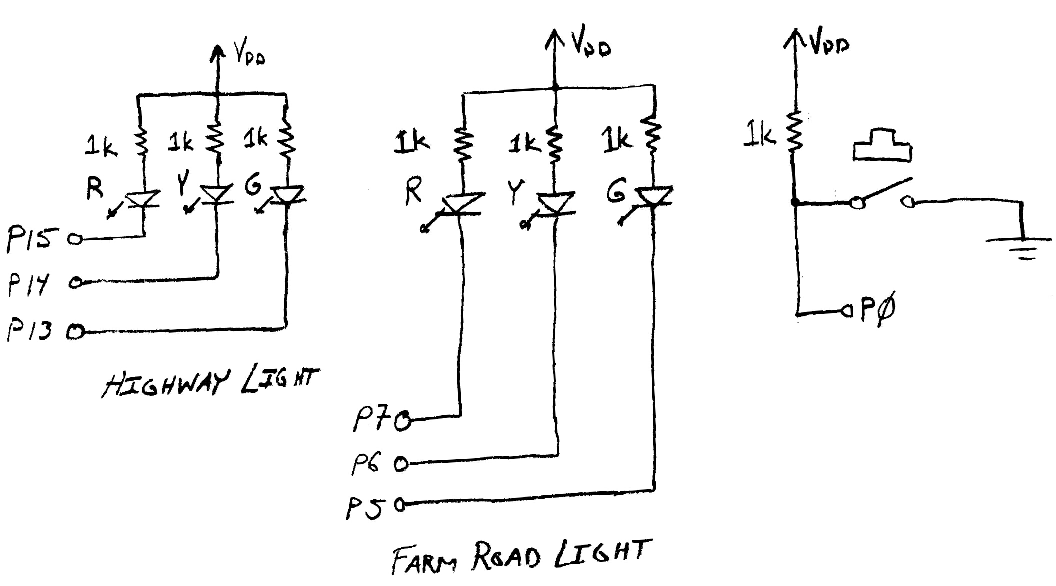
\includegraphics[width=.6\textwidth]{traffic-light-circuit.pdf}
\caption{Traffic Light Controller Circuit Diagram}
\label{traffic-light-circuit}
\end{figure}

The control flow chart for the PBasic program is shown in \hyperref[traffic-light-flowchart]{figure \ref{traffic-light-flowchart}}.

\begin{figure}[ht]
\centering
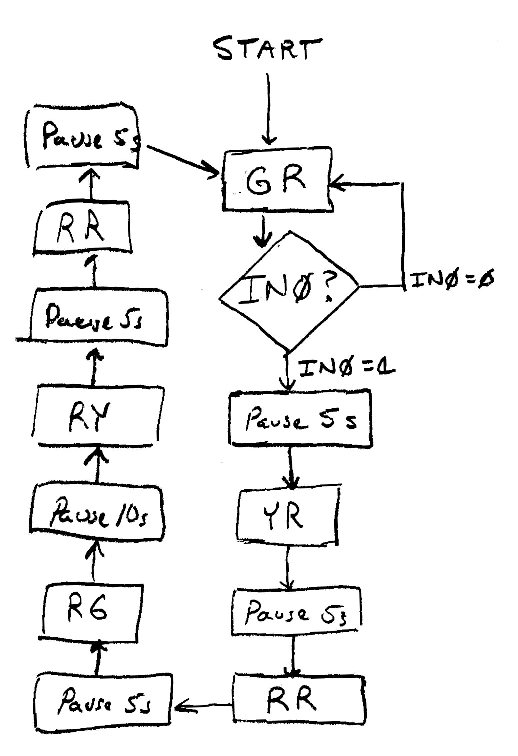
\includegraphics[width=0.3\textwidth]{traffic-light-flowchart.pdf}
\caption{Traffic Light Controller Flowchart}
\label{traffic-light-flowchart}
\end{figure}

\subsection{Jeopardy Style Game}

I designed the circuit for the Jeopardy game similarly to the traffic light controller.
Each LED or pushbutton switch has a $1k\Omega$ current limiting resistor and is configured active low.
The circuit diagram for the Jeopardy game is shown in \hyperref[jeopardy-circuit]{figure \ref{jeopardy-circuit}}.

\begin{figure}[h!]
\centering
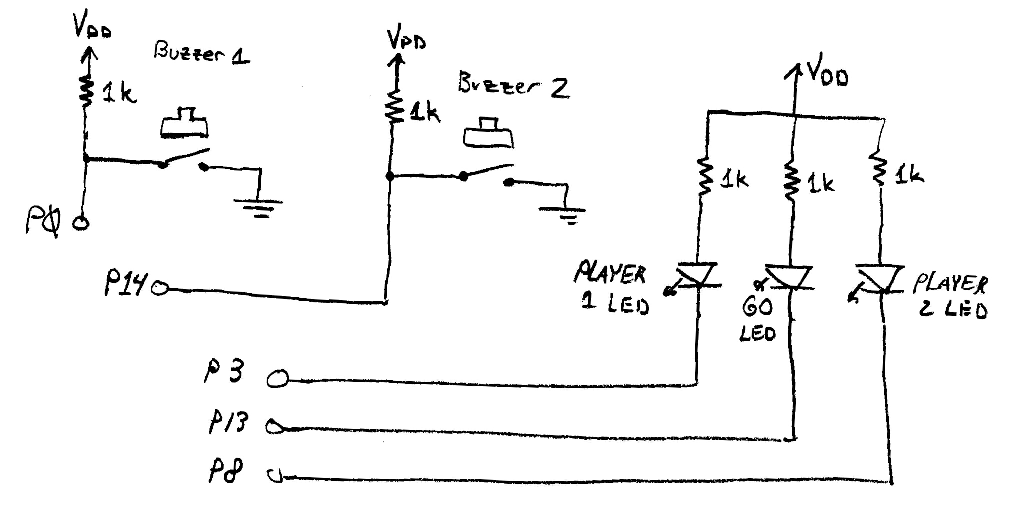
\includegraphics[width=0.7\textwidth]{jeopardy-circuit.pdf}
\caption{Jeopardy Circuit Diagram}
\label{jeopardy-circuit}
\end{figure}

The jeopardy game was more complicated than the traffic light controller,
but only from a software perspective--not hardware.

I used the random function to generate a random delay time before the game begins,
passing in the previous game's reaction time as a seed value so that the same
pseudorandom sequence is not repeated every game.

Once the game begins the microcontroller executes a tight loop that does checks the pushbuttons
for a victor and then increments a react\_cycles variable.
When the first player buzzes in, the appropriate LED lights up and their reaction
time is calculated from the number of cycles and the closest integer to the loop iteration time.
This value is printed to the debug terminal.

The control flow chart for the PBasic program is shown in \hyperref[jeopardy-flowchart]{figure \ref{jeopardy-flowchart}}.

\begin{figure}[ht]
\centering
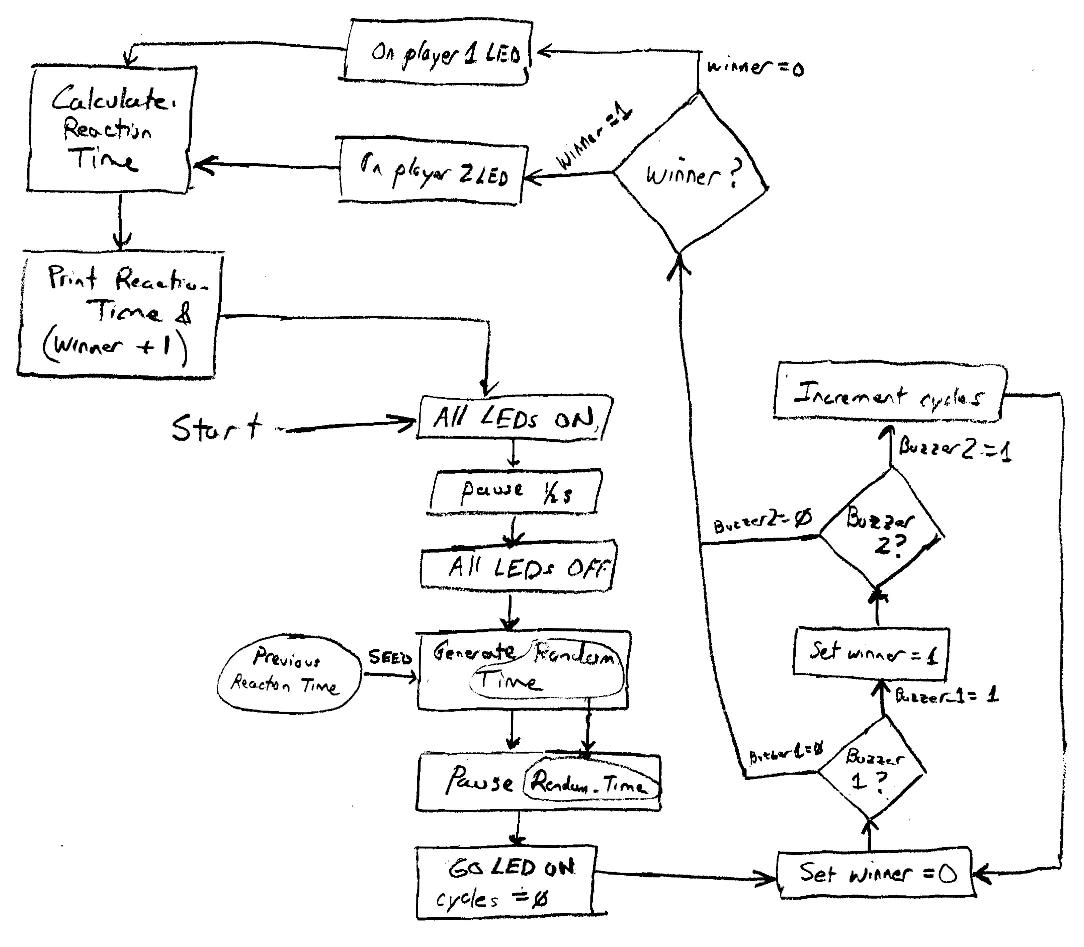
\includegraphics[width=0.7\textwidth]{jeopardy-flowchart.pdf}
\caption{Jeopardy-Like Game Flowchart}
\label{jeopardy-flowchart}
\end{figure}

\section{Expected Results}

I expected both circuits to behave according to the problem statements.

\section{Experiment and Design Revisions}

\subsection{Traffic Light Controller}

This circuit and code worked like a charm.
No revisions had to be made, but I did restyle the code to look more like C with boolean algebra.

\subsection{Jeopardy Game}

I really did not want to have two sets of Debug statements, depending on the winner.
However, using only one Debug statement and storing the winner in a bit variable proved more difficult than I anticipated.

It was difficult to generate the boolean algebra statements for turning on the appropriate LEDs,
mostly because PBasic sucks and doesn't even have a complete set of boolean operators.

So reducing to one set of Debut statements and only a single goto location proved more difficult,
but I think it was worth the change for code brevity.

\section{Observations}

Both circuits worked as expected, and photos of the working boards are shown in
\hyperref[traffic-light]{figure \ref{traffic-light}}
and \hyperref[jeopardy-board]{figure \ref{jeopardy-board}}.
A screenshot of the Debug terminal for the Jeopardy board is shown in figure \ref{jeopardy-screenshot}.

\begin{figure}
\centering
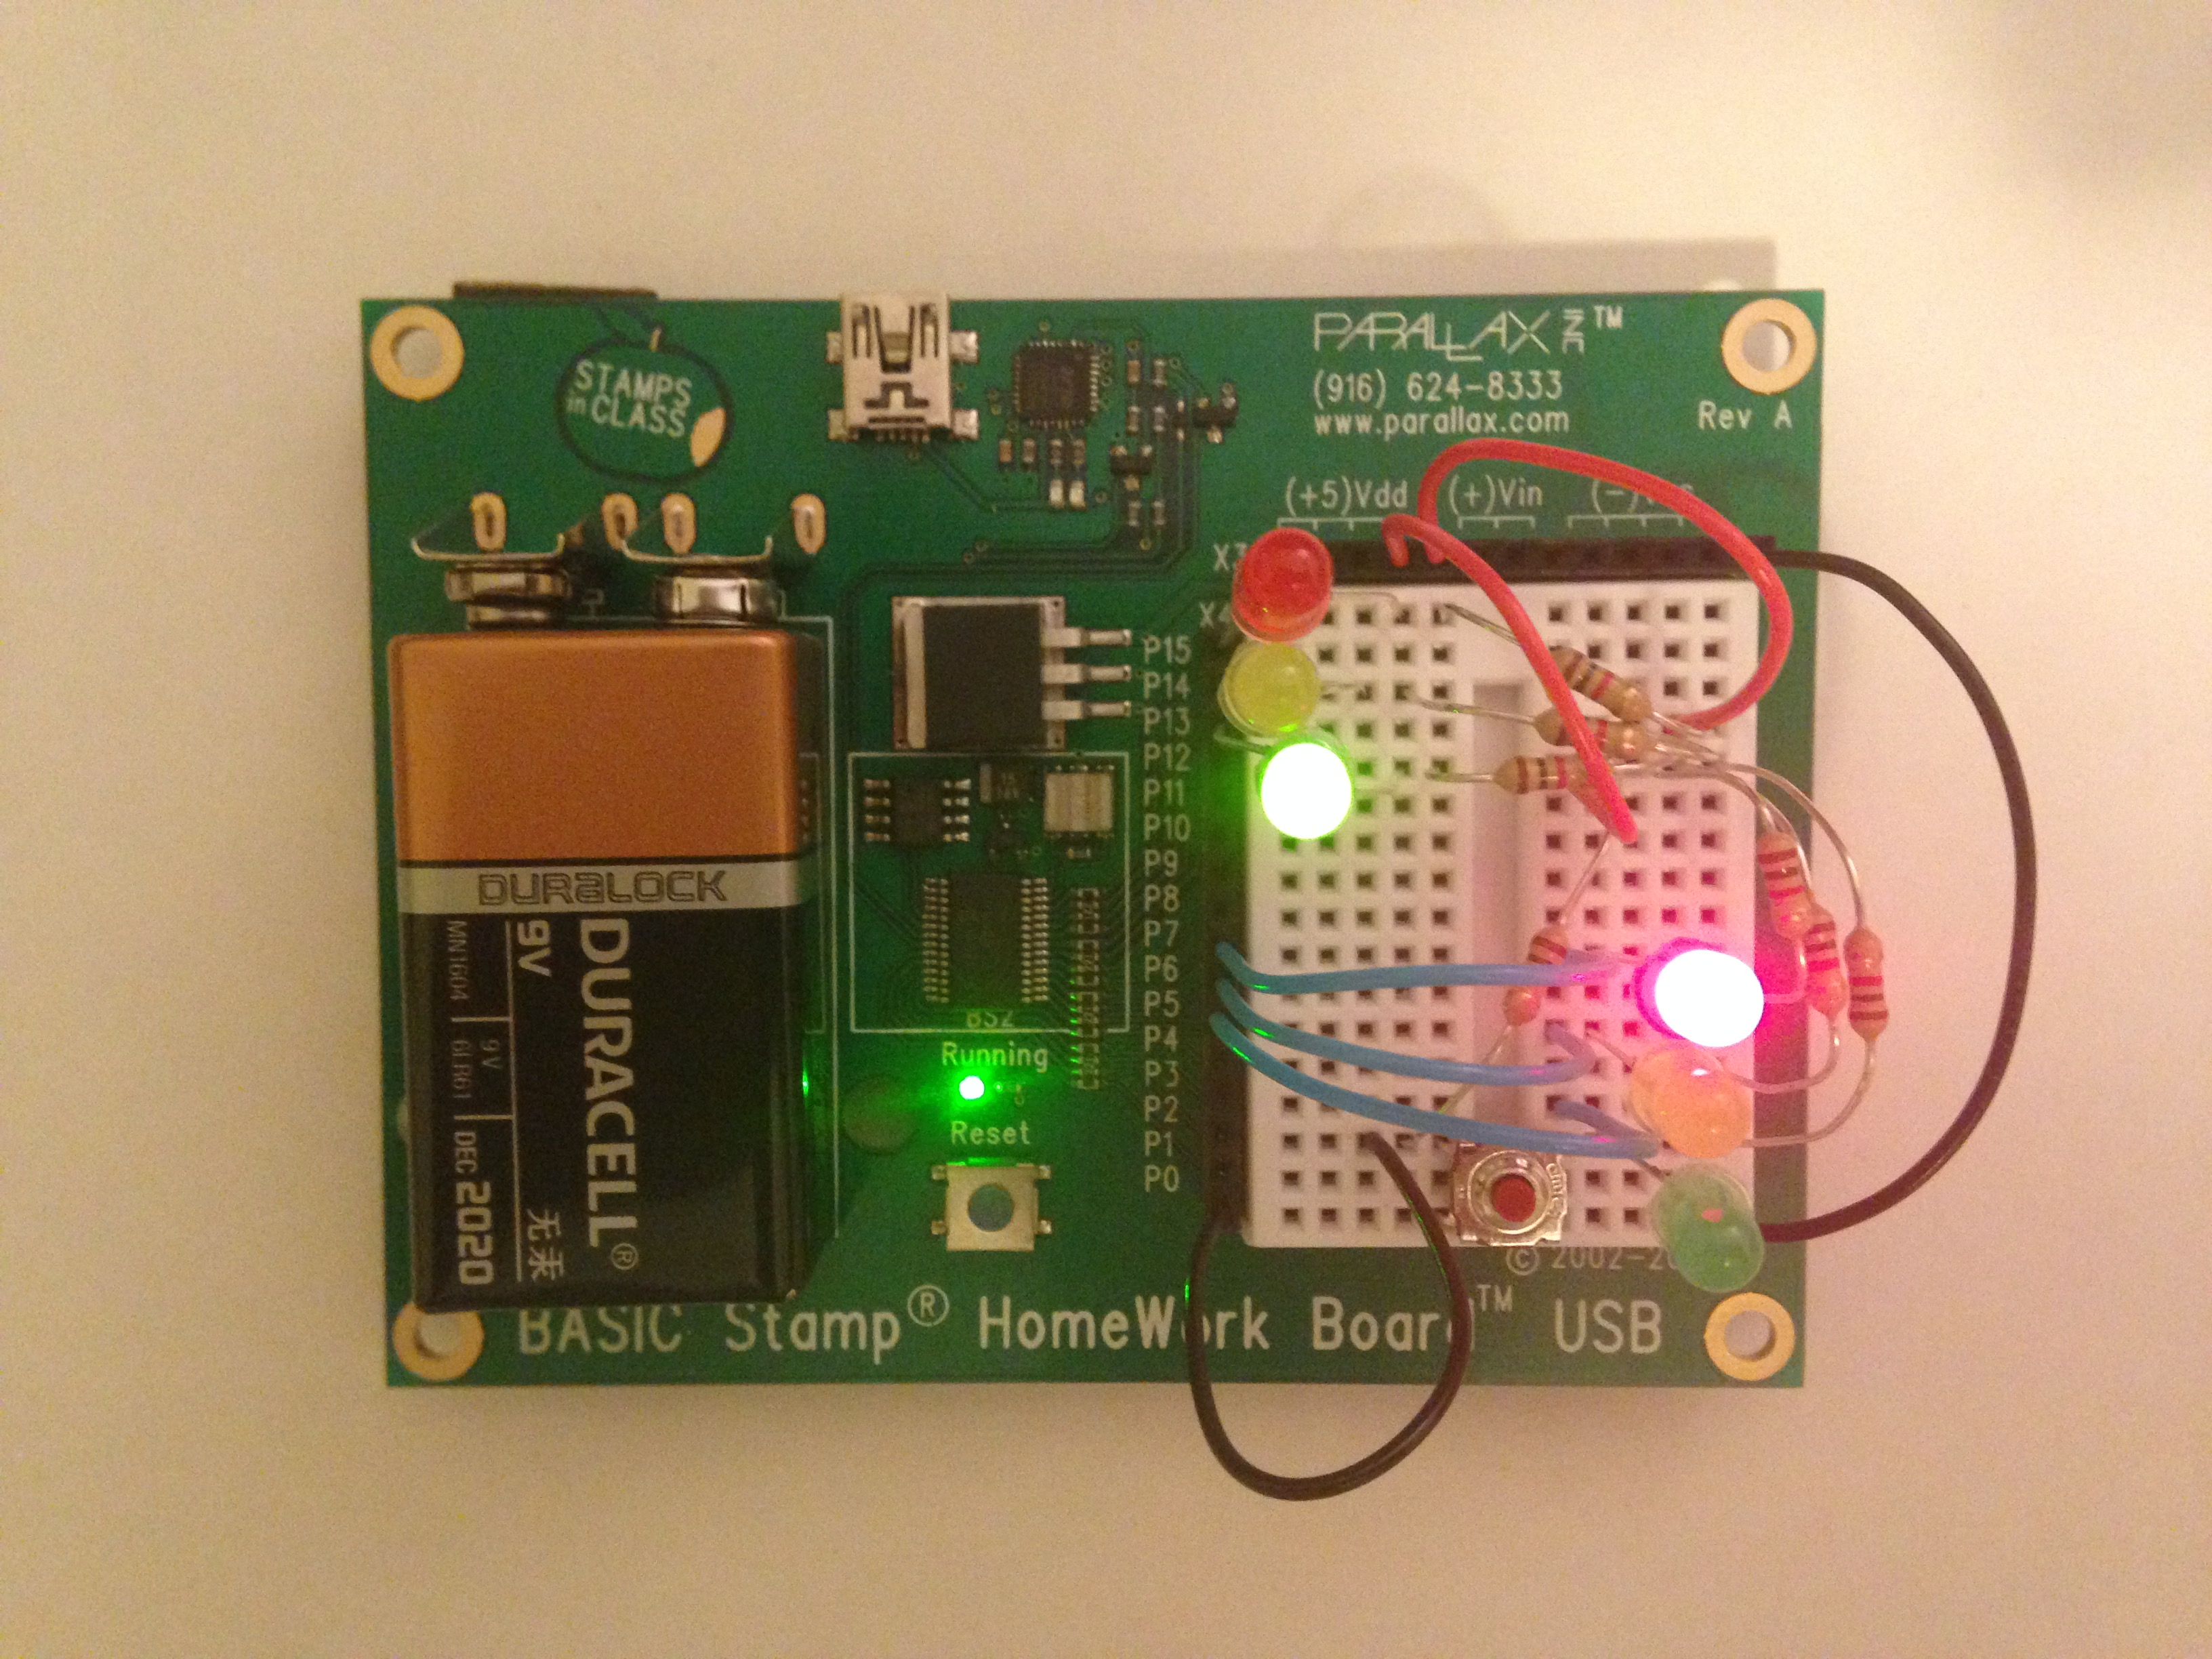
\includegraphics[width=0.6\textwidth]{traffic-light.jpg}
\caption{Traffic Light Controller Circuit}
\label{traffic-light}
\end{figure}

\begin{figure}
\centering
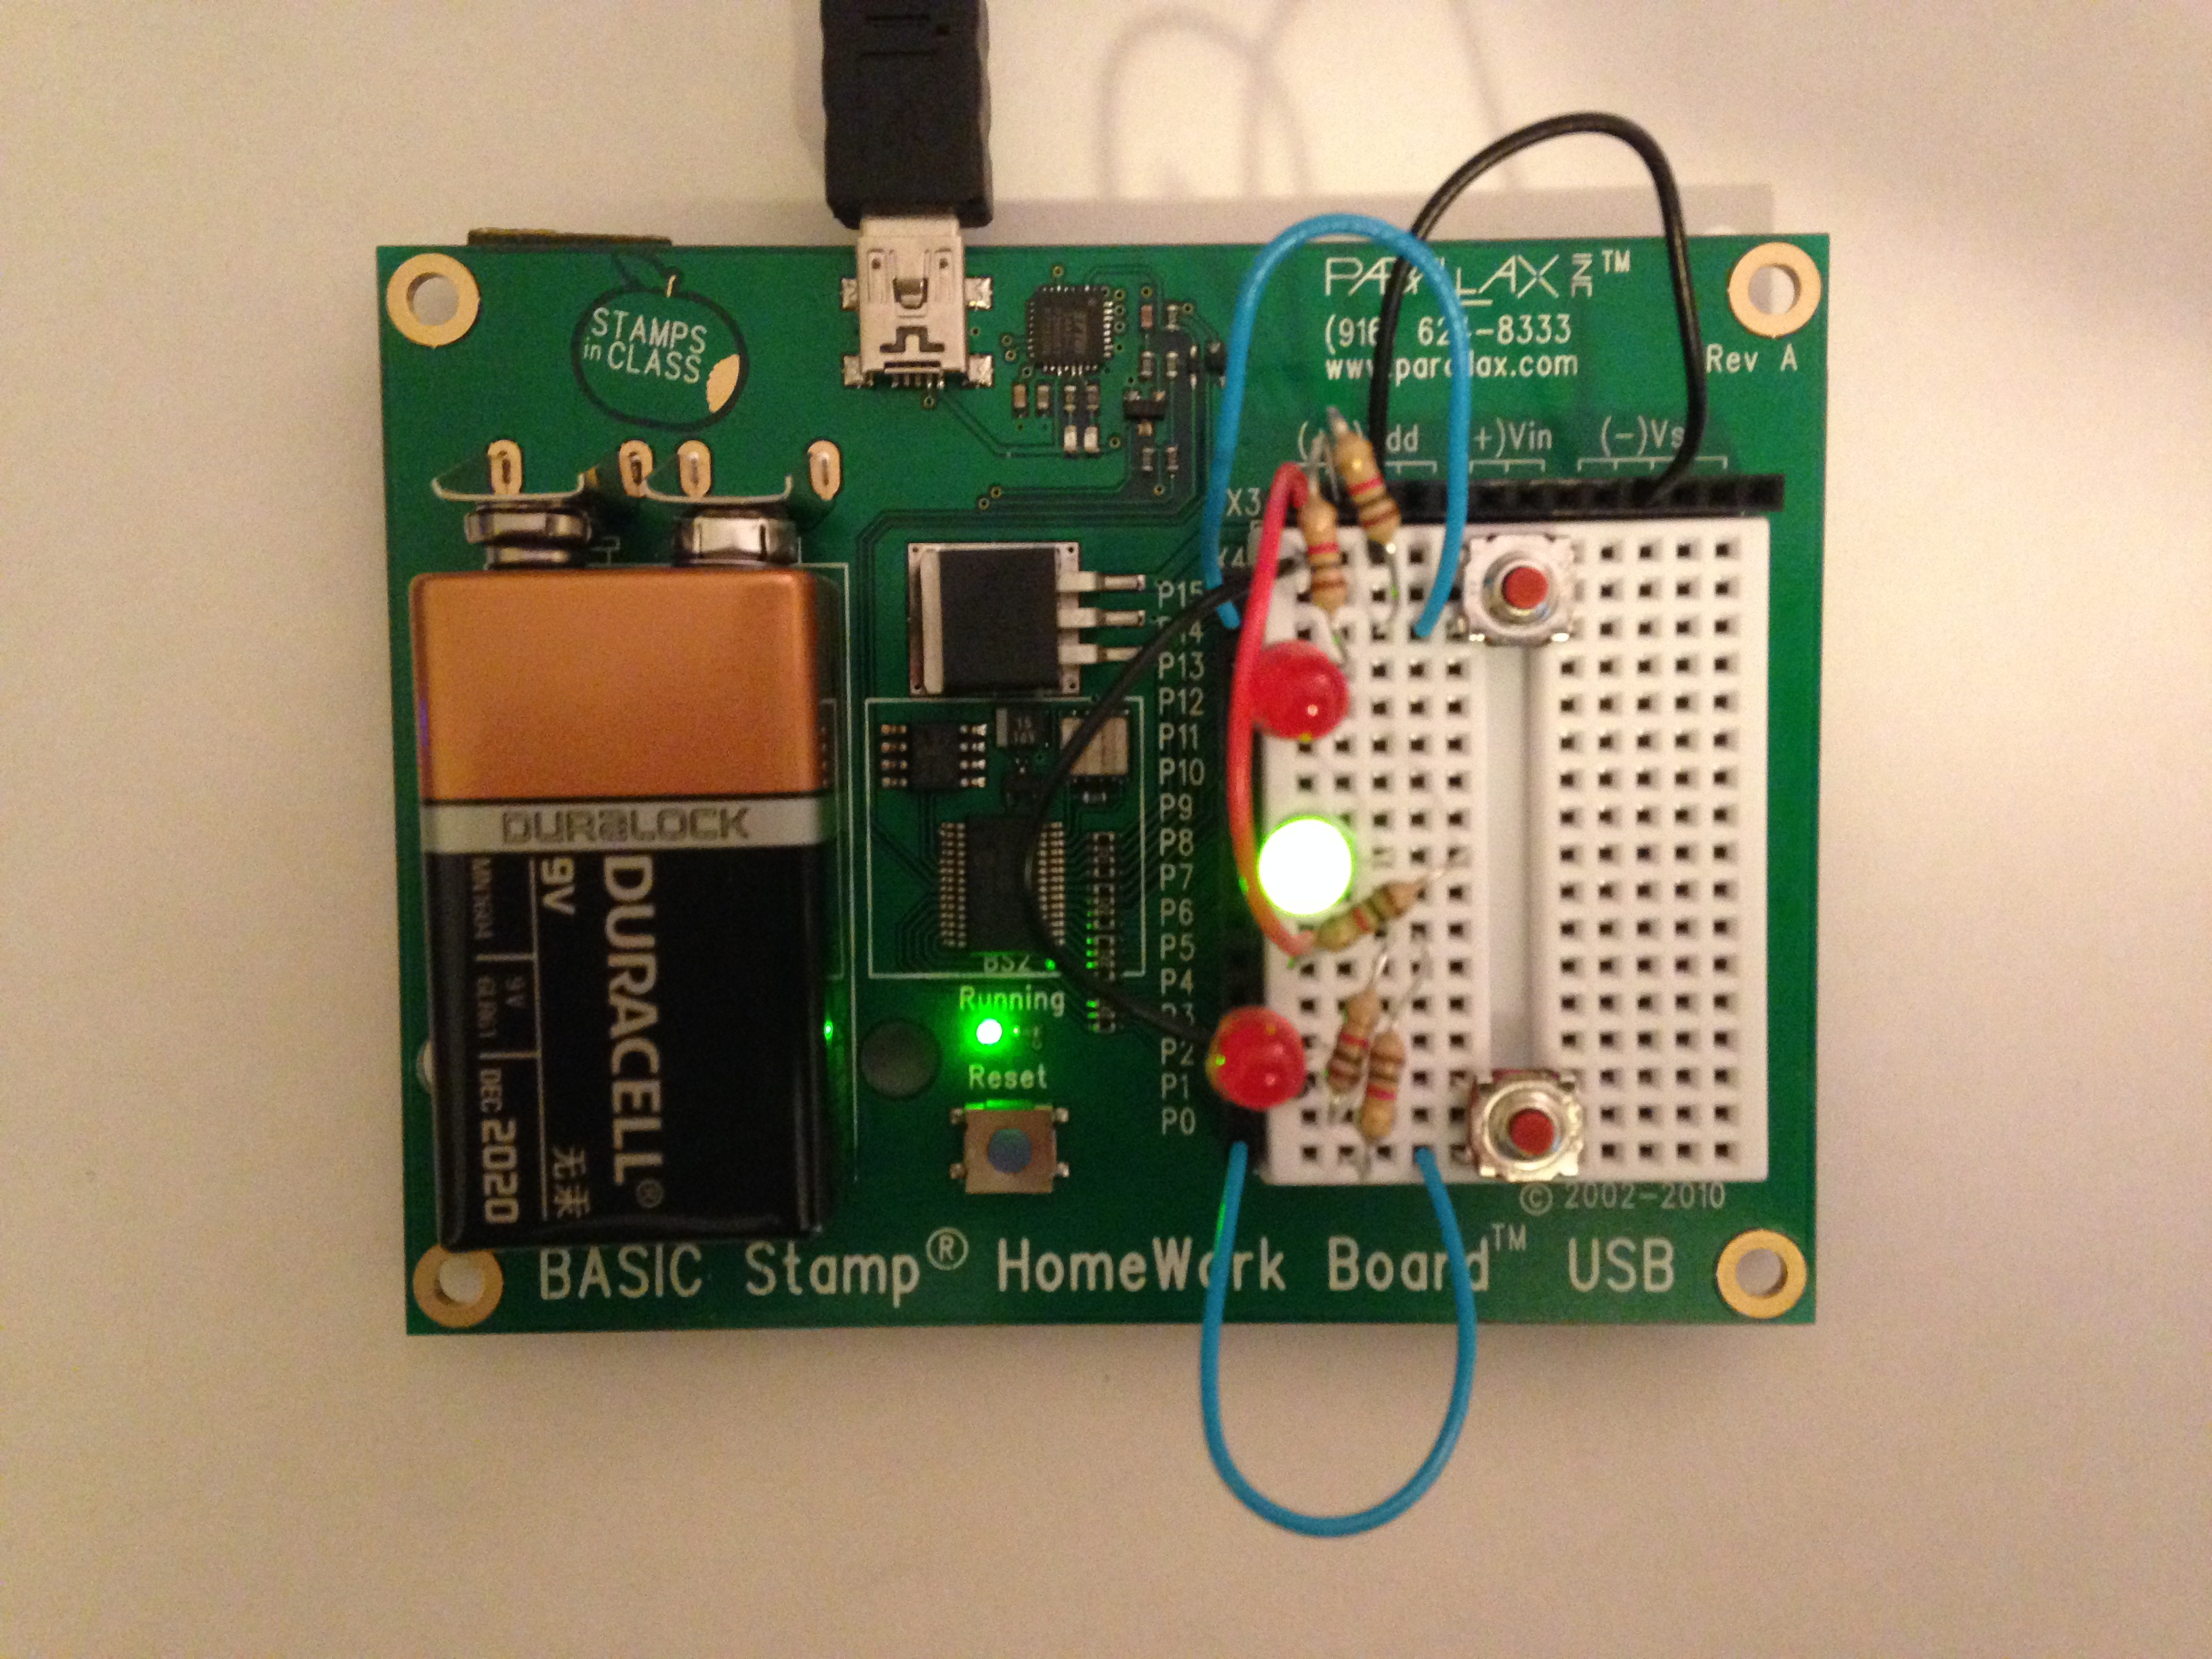
\includegraphics[width=0.6\textwidth]{jeopardy-board.jpg}
\caption{Jeopardy Game Circuit}
\label{jeopardy-board}
\end{figure}

\begin{figure}
\centering
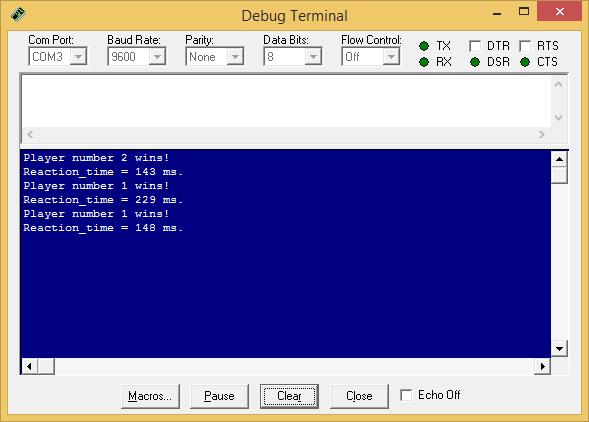
\includegraphics[width=0.75\textwidth]{jeopardy-screenshot.jpg}
\caption{Screenshot of Jeopardy Debug Terminal with Reaction Times}
\label{jeopardy-debug}
\end{figure}

\section{Discussion}

This lab really revealed a major flaw of the Stamp Basic board:
the fact that running an interpreter prevents you from knowing exact timing.
If we were writing code directly for PIC, we could no the clock rate and write some
assembly inside the reaction time loop--and therby no the exact number of clock cycles
and the clock rate.

I have a low opinion of the Stamp Basic board right now, at least compared to other
microcontrollers. This week I complain about not having control of clock cycles or there being
a clock variable that is accessable. Next weeks' dissatisfaction preview: no ADC on board.

\section{Exercises}

There were no exercises given.

\clearpage
\section{Programs}

\subsection{Traffic Light Controller}
\begingroup
\fontsize{10pt}{12pt}

\verbatiminput{Traffic-Controller.bs2}

\endgroup

\clearpage
\subsection{Jeopardy Style Game}
\begingroup
\fontsize{9pt}{11pt}

\verbatiminput{Jeopardy.bs2}

\endgroup

\end{document}
